%%%%%%%%%%%%%%%%%%%%%%%%%%%%%%%%%%%%%%%%%%%%%%%%%%%%%%%%%%%%%%%%%%%%%%
% 
% 	Template for Producing ASP-DAC 2018 Proceedings
% 
%%%%%%%%%%%%%%%%%%%%%%%%%%%%%%%%%%%%%%%%%%%%%%%%%%%%%%%%%%%%%%%%%%%%%%
% History
% ??/??/?? Designed by Hiroaki Kunieda (ASP-DAC '97 Publication Chair)
% 09/22/97 Modified and small bug fixed by Masaharu Imai 
% 	   (ASP-DAC '98 Publication Chair)
% 11/02/98 Modified by Tsuyoshi Isshiki
% 	   (ASP-DAC 2000 TPS Secretary)
% 7/24/00 Modified by Kiyoharu Hamaguchi
% 	   (ASP-DAC 2001 Publication chair)
% 6/18/02 Modified by Kazutoshi Kobayashi
% 	   (ASP-DAC 2003 Publication Co-Chair)
% 5/27/03 Modified by Kiyoharu Hamaguchi
% 	   (ASP-DAC 2004 TPC secretary)
% 6/10/03 Modified by Kazutoshi Kobayashi for Latex2e
% 	   (ASP-DAC 2004 Publication Co-Chair)
% 6/01/05 Modified by Nozomu Togawa
% 	   (ASP-DAC 2006 Publication Chair)
% 6/01/06 Modified by Hiroyuki Ochi
% 	   (ASP-DAC 2007 Publication Chair)
% 5/30/08 Modified by Nozomu Togawa
% 	   (ASP-DAC 2009 Publication Co-Chair)
% 4/30/10 Modified by Masashi Imai
% 	   (ASP-DAC 2011 Publication Chair)
% 3/20/12 Modified by Masashi Imai
% 	   (ASP-DAC 2013 Publication Chair)
% 5/01/14 Modified by Masashi Imai
% 	   (ASP-DAC 2015 Publication Chair)
% 4/24/16 Modified by Masashi Imai
% 	   (ASP-DAC 2017 Publication Chair)
% 2/06/17 Modified by Jongeun Lee
% 	   (ASP-DAC 2018 Publication Chair)
%%%%%%%%%%%%%%%%%%%%%%%%%%%%%%%%%%%%%%%%%%%%%%%%%%%%%%%%%%%%%%%%%%%%%%
% If you have any problem, please contact ASP-DAC 2018 Publication
% Chair by E-mail at "jlee@unist.ac.kr.''
%%%%%%%%%%%%%%%%%%%%%%%%%%%%%%%%%%%%%%%%%%%%%%%%%%%%%%%%%%%%%%%%%%%%%%
%
\documentclass[twocolumn]{article}
%% If you use dvips and ps2pdf, please use Postscript font 
%% and uncomment the line below.
%%\usepackage{times}
\usepackage[dvipdfmx]{graphicx}
\pagestyle{empty}
%set paper size
%for A4 paper
\topmargin      29mm    %bottom margin 30mm
\oddsidemargin  15mm    %left & right margin 15mm

%for 8 1/2" x 11" paper paper, use the following definition
%\topmargin     17mm    %bottom margin 24mm
%\oddsidemargin 18mm    %left margin 18mm & right margin 17mm

%text sizes
\textwidth  180mm
\textheight 238mm
\columnsep  5.0mm
\parindent  3.5mm

%misc parameters
\headsep 0mm  \headheight 0mm
\footskip 18mm
%\footheight 6mm

%conversion to values for LaTeX
\advance\topmargin-1in\advance\oddsidemargin-1in
\evensidemargin\oddsidemargin

\makeatletter
%as Latex considers descenders in its calculation of interline spacing,
%to get 12 point spacing for normalsize text, must set it to 10 points
\def\@normalsize{\@setsize\normalsize{12pt}\xpt\@xpt
\abovedisplayskip 10pt plus2pt minus5pt\belowdisplayskip \abovedisplayskip
\abovedisplayshortskip \z@ plus3pt\belowdisplayshortskip 6pt plus3pt
minus3pt\let\@listi\@listI}

%interline spaceing and title font for section
\def\section{\@startsection {section}{1}{\z@}{20pt plus 2pt minus 2pt}
{8pt plus 2pt minus 2pt}{\centering\normalsize\sc
\edef\@svsec{\thesection.\ }}}
\def\thesection{\Roman{section}}

%interline spacing and title font for subsection
\def\subsection{\@startsection {subsection}{2}{\z@}{16pt plus 2pt minus 2pt}
{6pt plus 2pt minus 2pt}{\normalsize\sl
\edef\@svsec{\thesubsection.\ }}}
\def\thesubsection{\Alph{subsection}}

%figures/tables captions
\long\def\@makecaption#1#2{
\vskip10pt\begin{center} #1 #2 \end{center}\par\vskip 1pt}
\def\fnum@figure{\raggedright{\footnotesize Fig. \thefigure }.%
\footnotesize}
\def\fnum@table{\footnotesize TABLE \thetable\\\footnotesize\sc}
\def\thetable{\Roman{table}}

\makeatother

\renewcommand{\floatpagefraction}{0.99}

%%%%%%%%%%%%%%%%%%%%%%%%%%%%%%%%%%%%%%%%%%%%%%%%%%%%%%%%%%%%%%%%%%%%%%%

\begin{document}
%date not printed
\date{}

%make title
\title{\Large\textbf{A Deep Neural Network Based Approach to Aestheticize Schematics}}%\\~\\
%\large\textbf{
%Preparation of Papers in Two-Column Format\\
%for the ASP-DAC 2018 (\LaTeX2e version)}}	% Modified by K. Kobayashi 18/06/02

%for single author
%\author{Center the Authors Names Here \\
%Center the Affiliations Here\\
%Center the City, Stats and Country Here\\
%{\small (it is your option if you want your entire address listed)}}

%for two authors
\author{Author 1 and Author 2}
\maketitle
\thispagestyle{empty}

{\small\textbf{Abstract---
This study proposes a novel method to combine schematic expression
and deep neural network to automatically aestheticize schematics.
Schematics are encoded to vectors so that the neural network can accept them.
Neural network is trained in supervised learning
with schematics and edit commands
which do not change the semantics of the schematics.
After training, schematics which are not a part of training data
are fed to trained neural network,
and the neural network makes given schematics aesthetic.
When trained with 33\% of all data,
the trained neural network has successfully aestheticized
95\% of schematics unused in traning.
}}

\section{Introduction}

Electronic design automation (EDA) has applied a positive feedback
for computer design by deploying computers themselves,
introducing an acceleration to growth of computing power
and achieving an exponential growth, along with Moore’s law.
Increasing the transistor count,
functionality of electronic devices and their complexity of design,
EDA has supported the development, by means of circuit simulator,
logic synthesis, high-level synthesis, automatic layout,
design rule checker, kinds of equivalence checkers,
automatic test pattern generator (ATPG), etc.
Those EDA tools handle topology information expressed as text data
called netlist which is easy for computer to deal with.
As well, output data from EDA are also text-based netlist,
which are result of automatic layout, result of parasitic extraction, etc.
Those text-based data often have to be manually analyzed
for debug or engineering change order (ECO),
but the analysis is error prone,
so schematics are often drawn down from netlist manually.
Schematic is more readable and understandable than text-based netlist,
so electronic circuitry is designed on schematic,
especially for analogue circuit.
Even though digital circuit is often designed
on hardware description language (HDL),
schematics are useful for complex and clock-cycle-timing-critical design,
e.g., pipeline \cite{ph}.
So far, methods to automatically generate schematic from netlist or HDL
have been proposed
\cite{nauts}
\cite{anshul}
\cite{fiduccia}
\cite{chun}
\cite{green}
\cite{tsung}
\cite{bogdan}.

Each of them focuses only on one of analog circuit,
gate level netlist of digital circuit
or more higher level HDL visualization.
And the best shape of schematic is likely to depend on
type of circuit, each project, or each individual.
Recently, interest to machine learning is raining,
and some studies have applied machine-learning-based techniques
to unprecedented realm of EDA \cite{fan} \cite{sourav}.
Among machine learning techniques,
deep neural network has demonstrated great performance
in application of recognizing field data
expanded on 2-dimensional space,
e.g., bitmap image or board game field \cite{nips} \cite{alphago}.

This study proposes a novel method to combine schematic expression
which is another 2-dimensional field data
and deep neural network to automatically manipulate schematics
and to achieve human-readable ones, based on its training result.
Schematics are encoded to vectors so that the neural network can accept them.
The encoded schematics and corresponding preferred schematic edit commands,
which are also encoded and do not change semantics of schematics,
are given as training data.
After training, schematics which are not a part of training data
are fed to trained neural network,
and the neural network makes given schematics aesthetic.

\section{Concept}

\begin{figure}[!tb]
 \begin{center}
  \begin{minipage}{\hsize}
   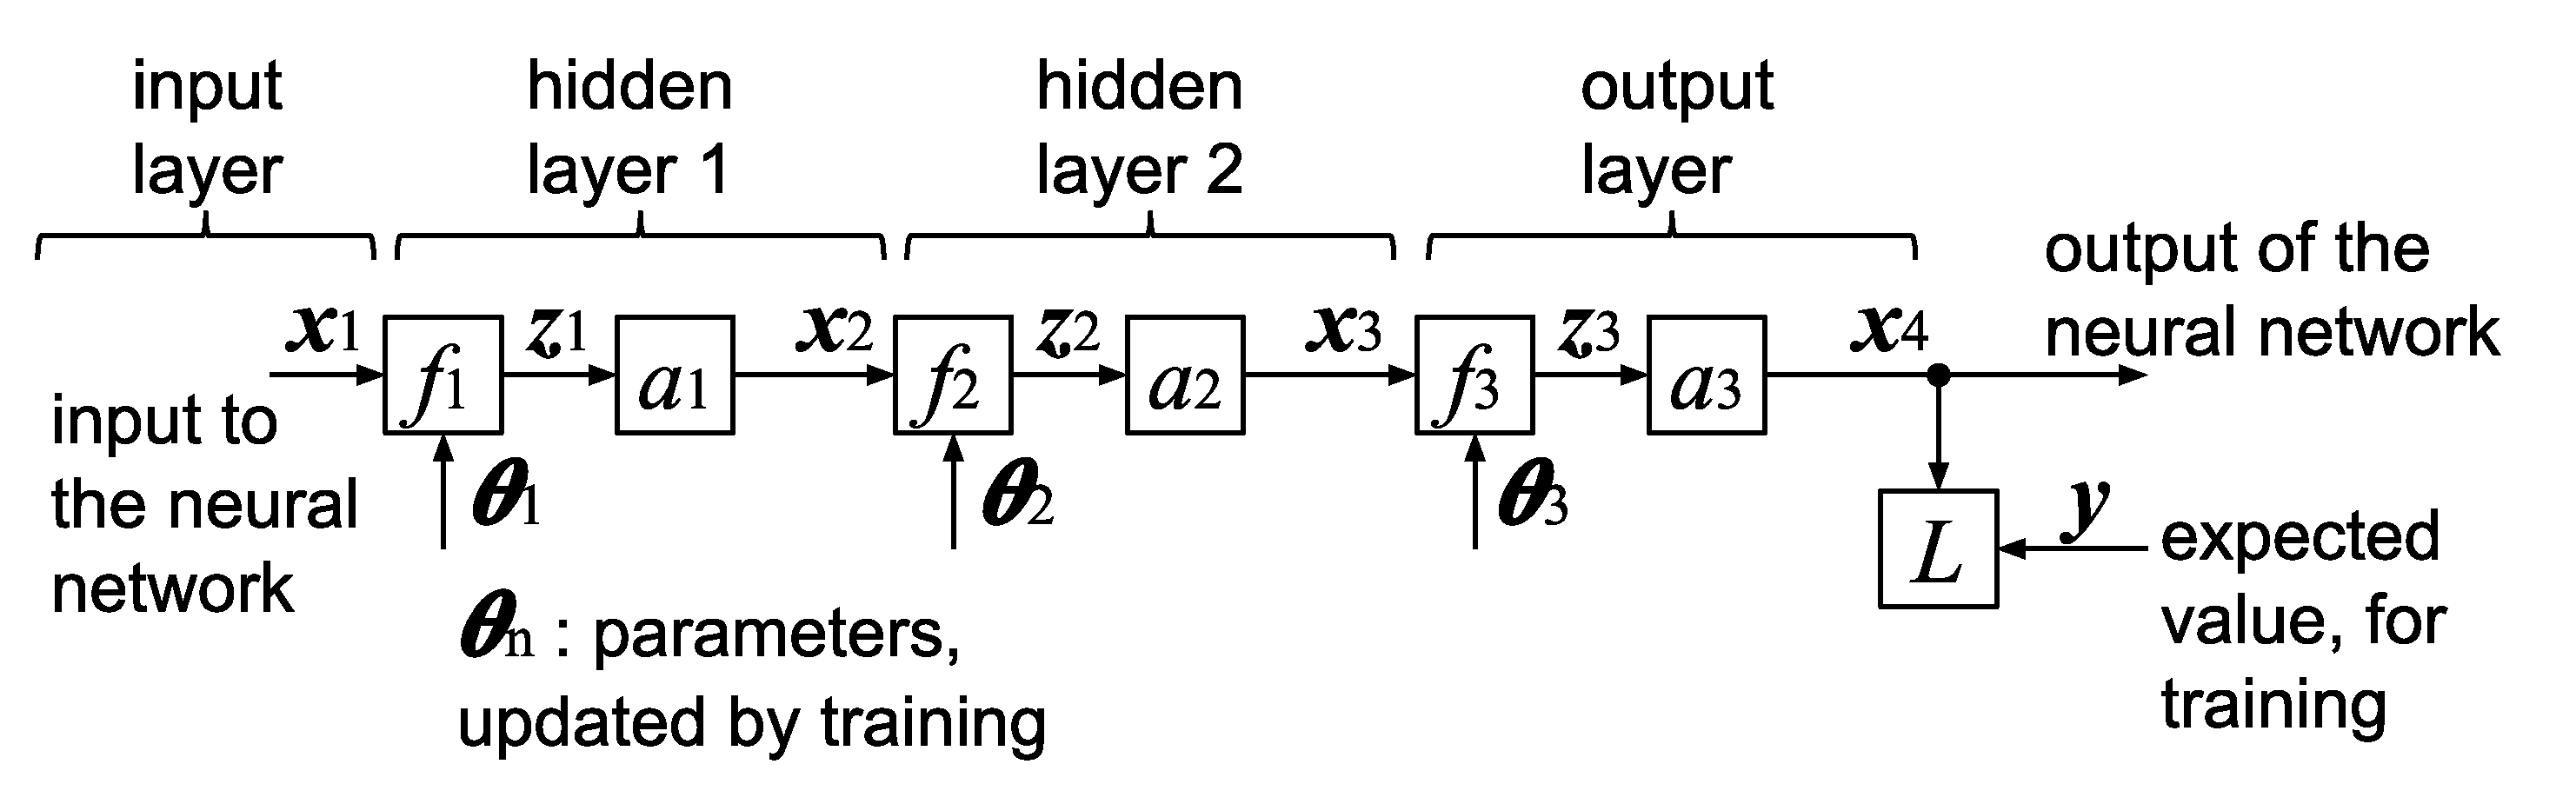
\includegraphics[width=\hsize]{fig/deep_feedforward_01.eps}
   \caption{deep feedforward network}
   \label{fig:deep_feedforward}
  \end{minipage}
 \end{center}
\end{figure}

\begin{figure}[!tb]
 \begin{center}
  \begin{minipage}{\hsize}
   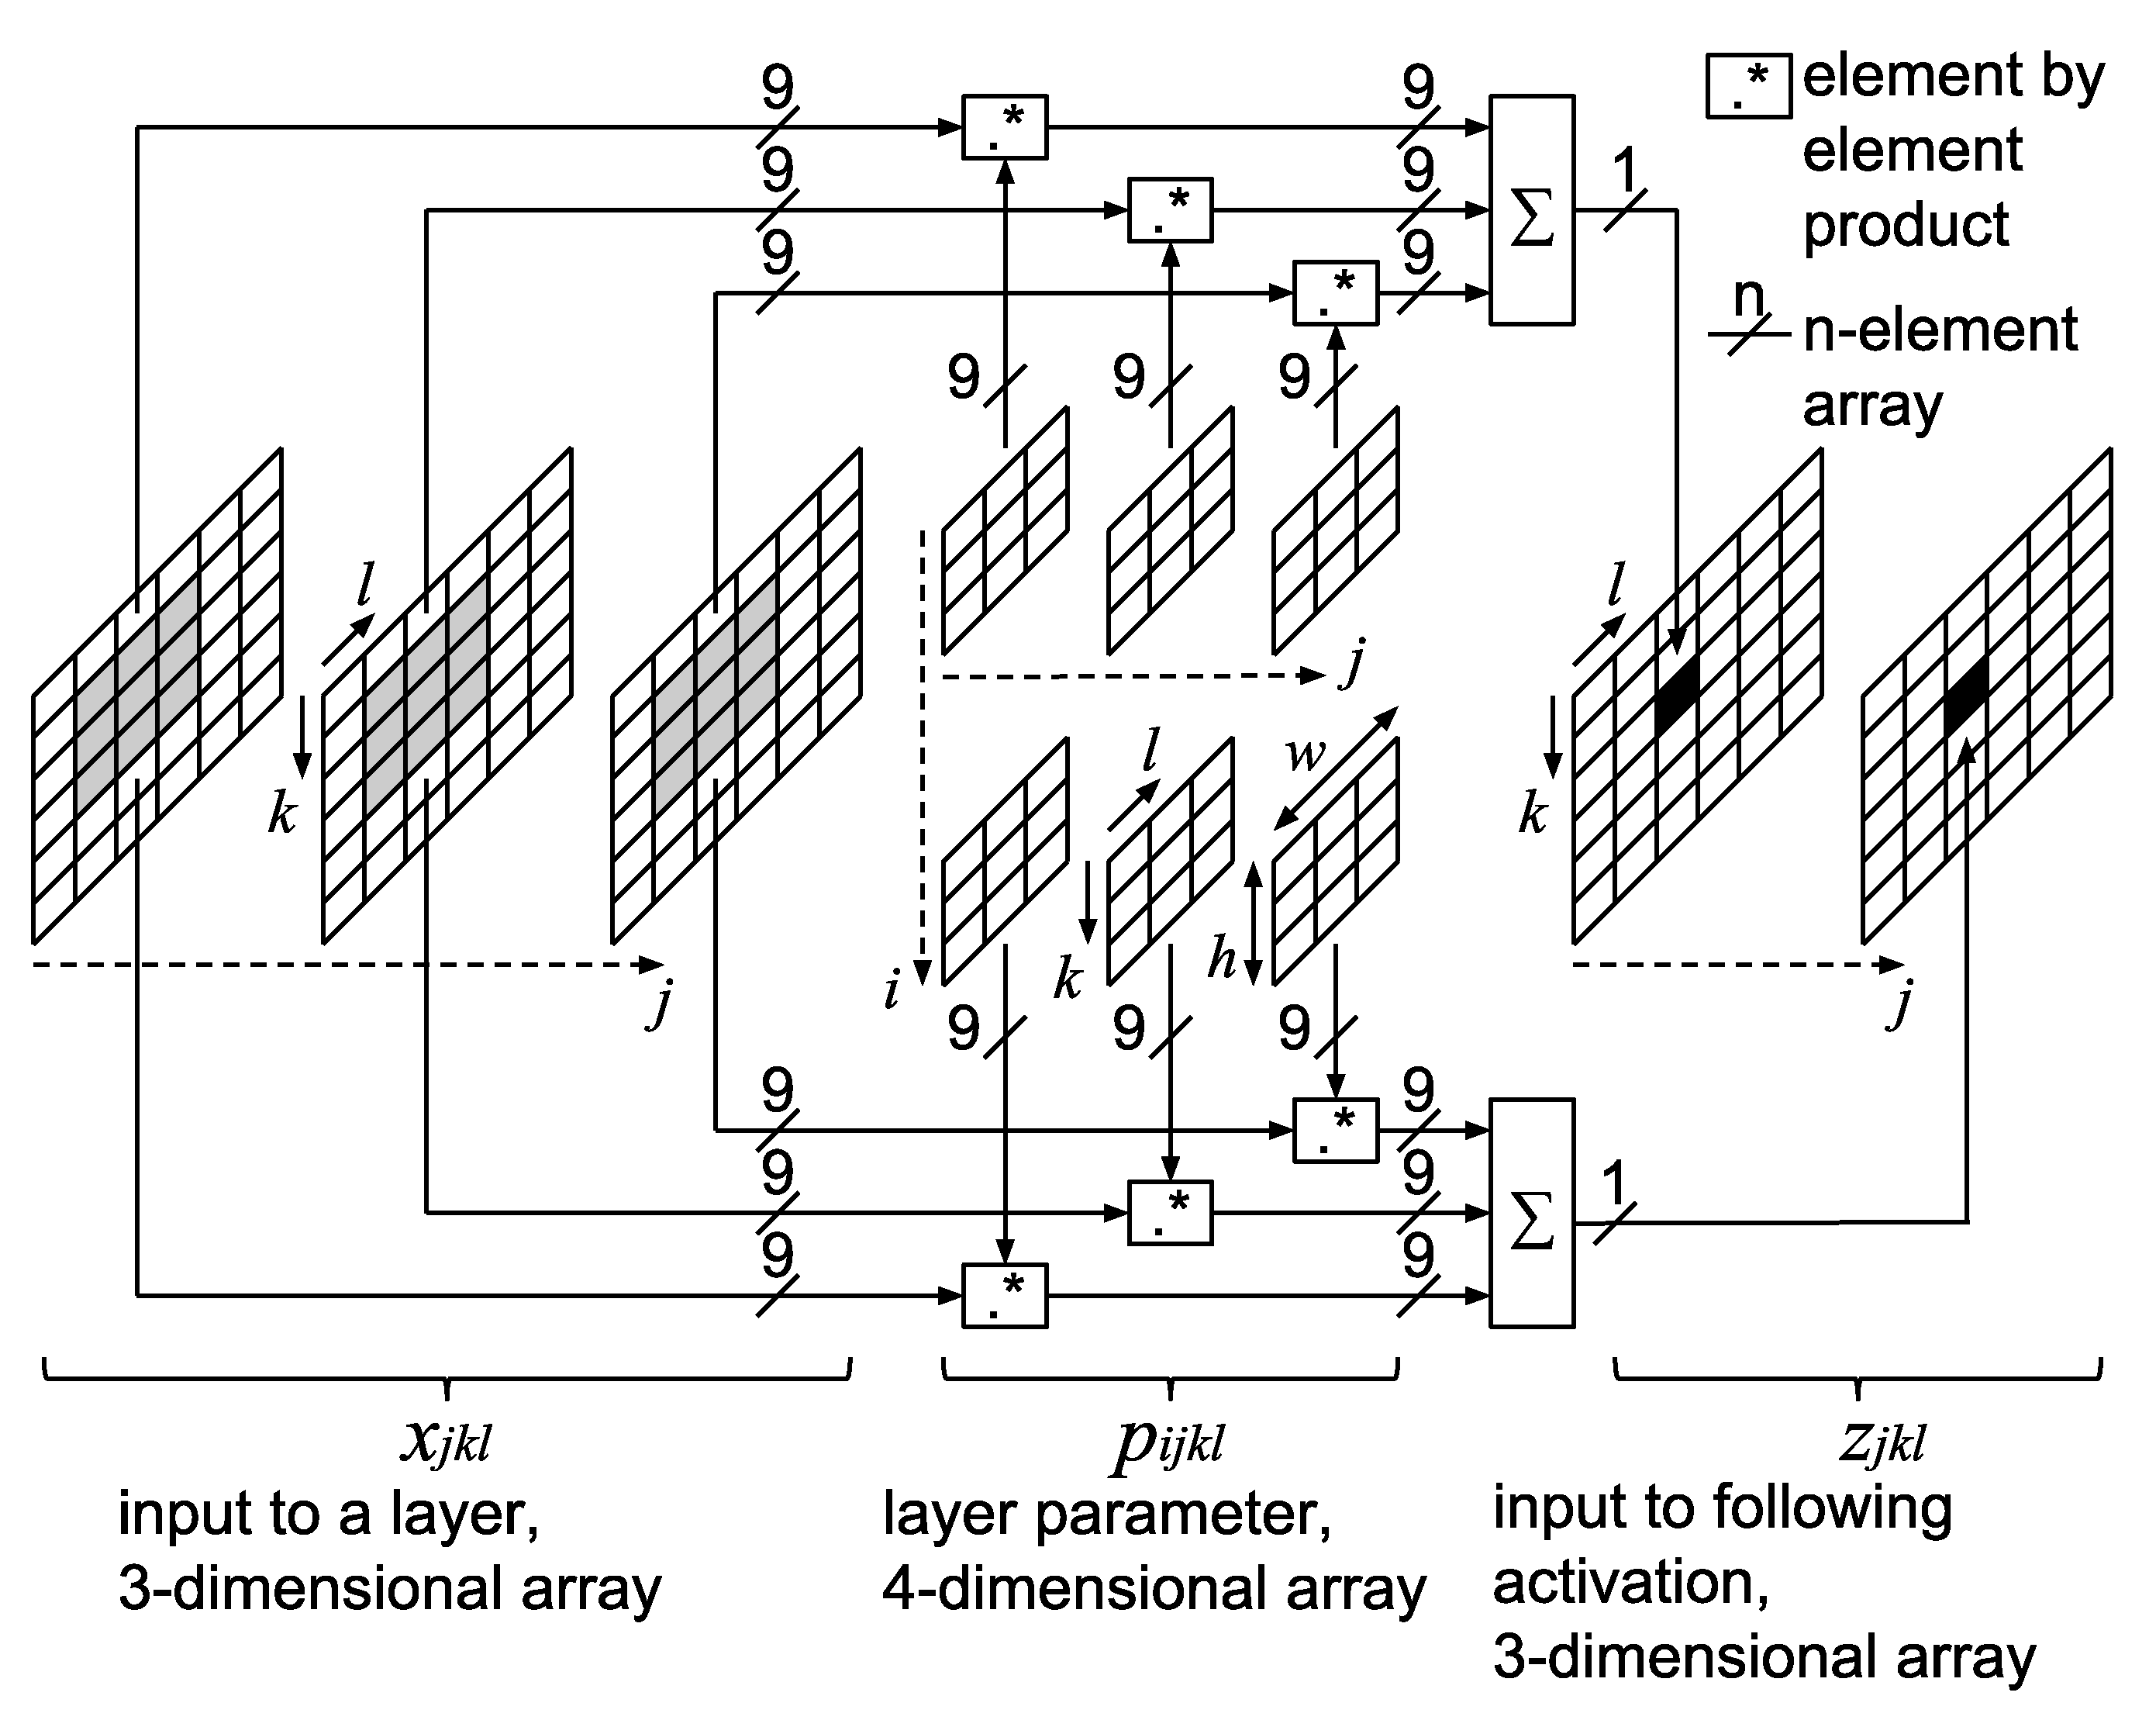
\includegraphics[width=\hsize]{fig/layer_convolutional_02.eps}
   \caption{convolutional layer}
   \label{fig:layer_convolutional}
  \end{minipage}
 \end{center}
\end{figure}

\begin{figure}[!tb]
 \begin{center}
  \begin{minipage}{\hsize}
   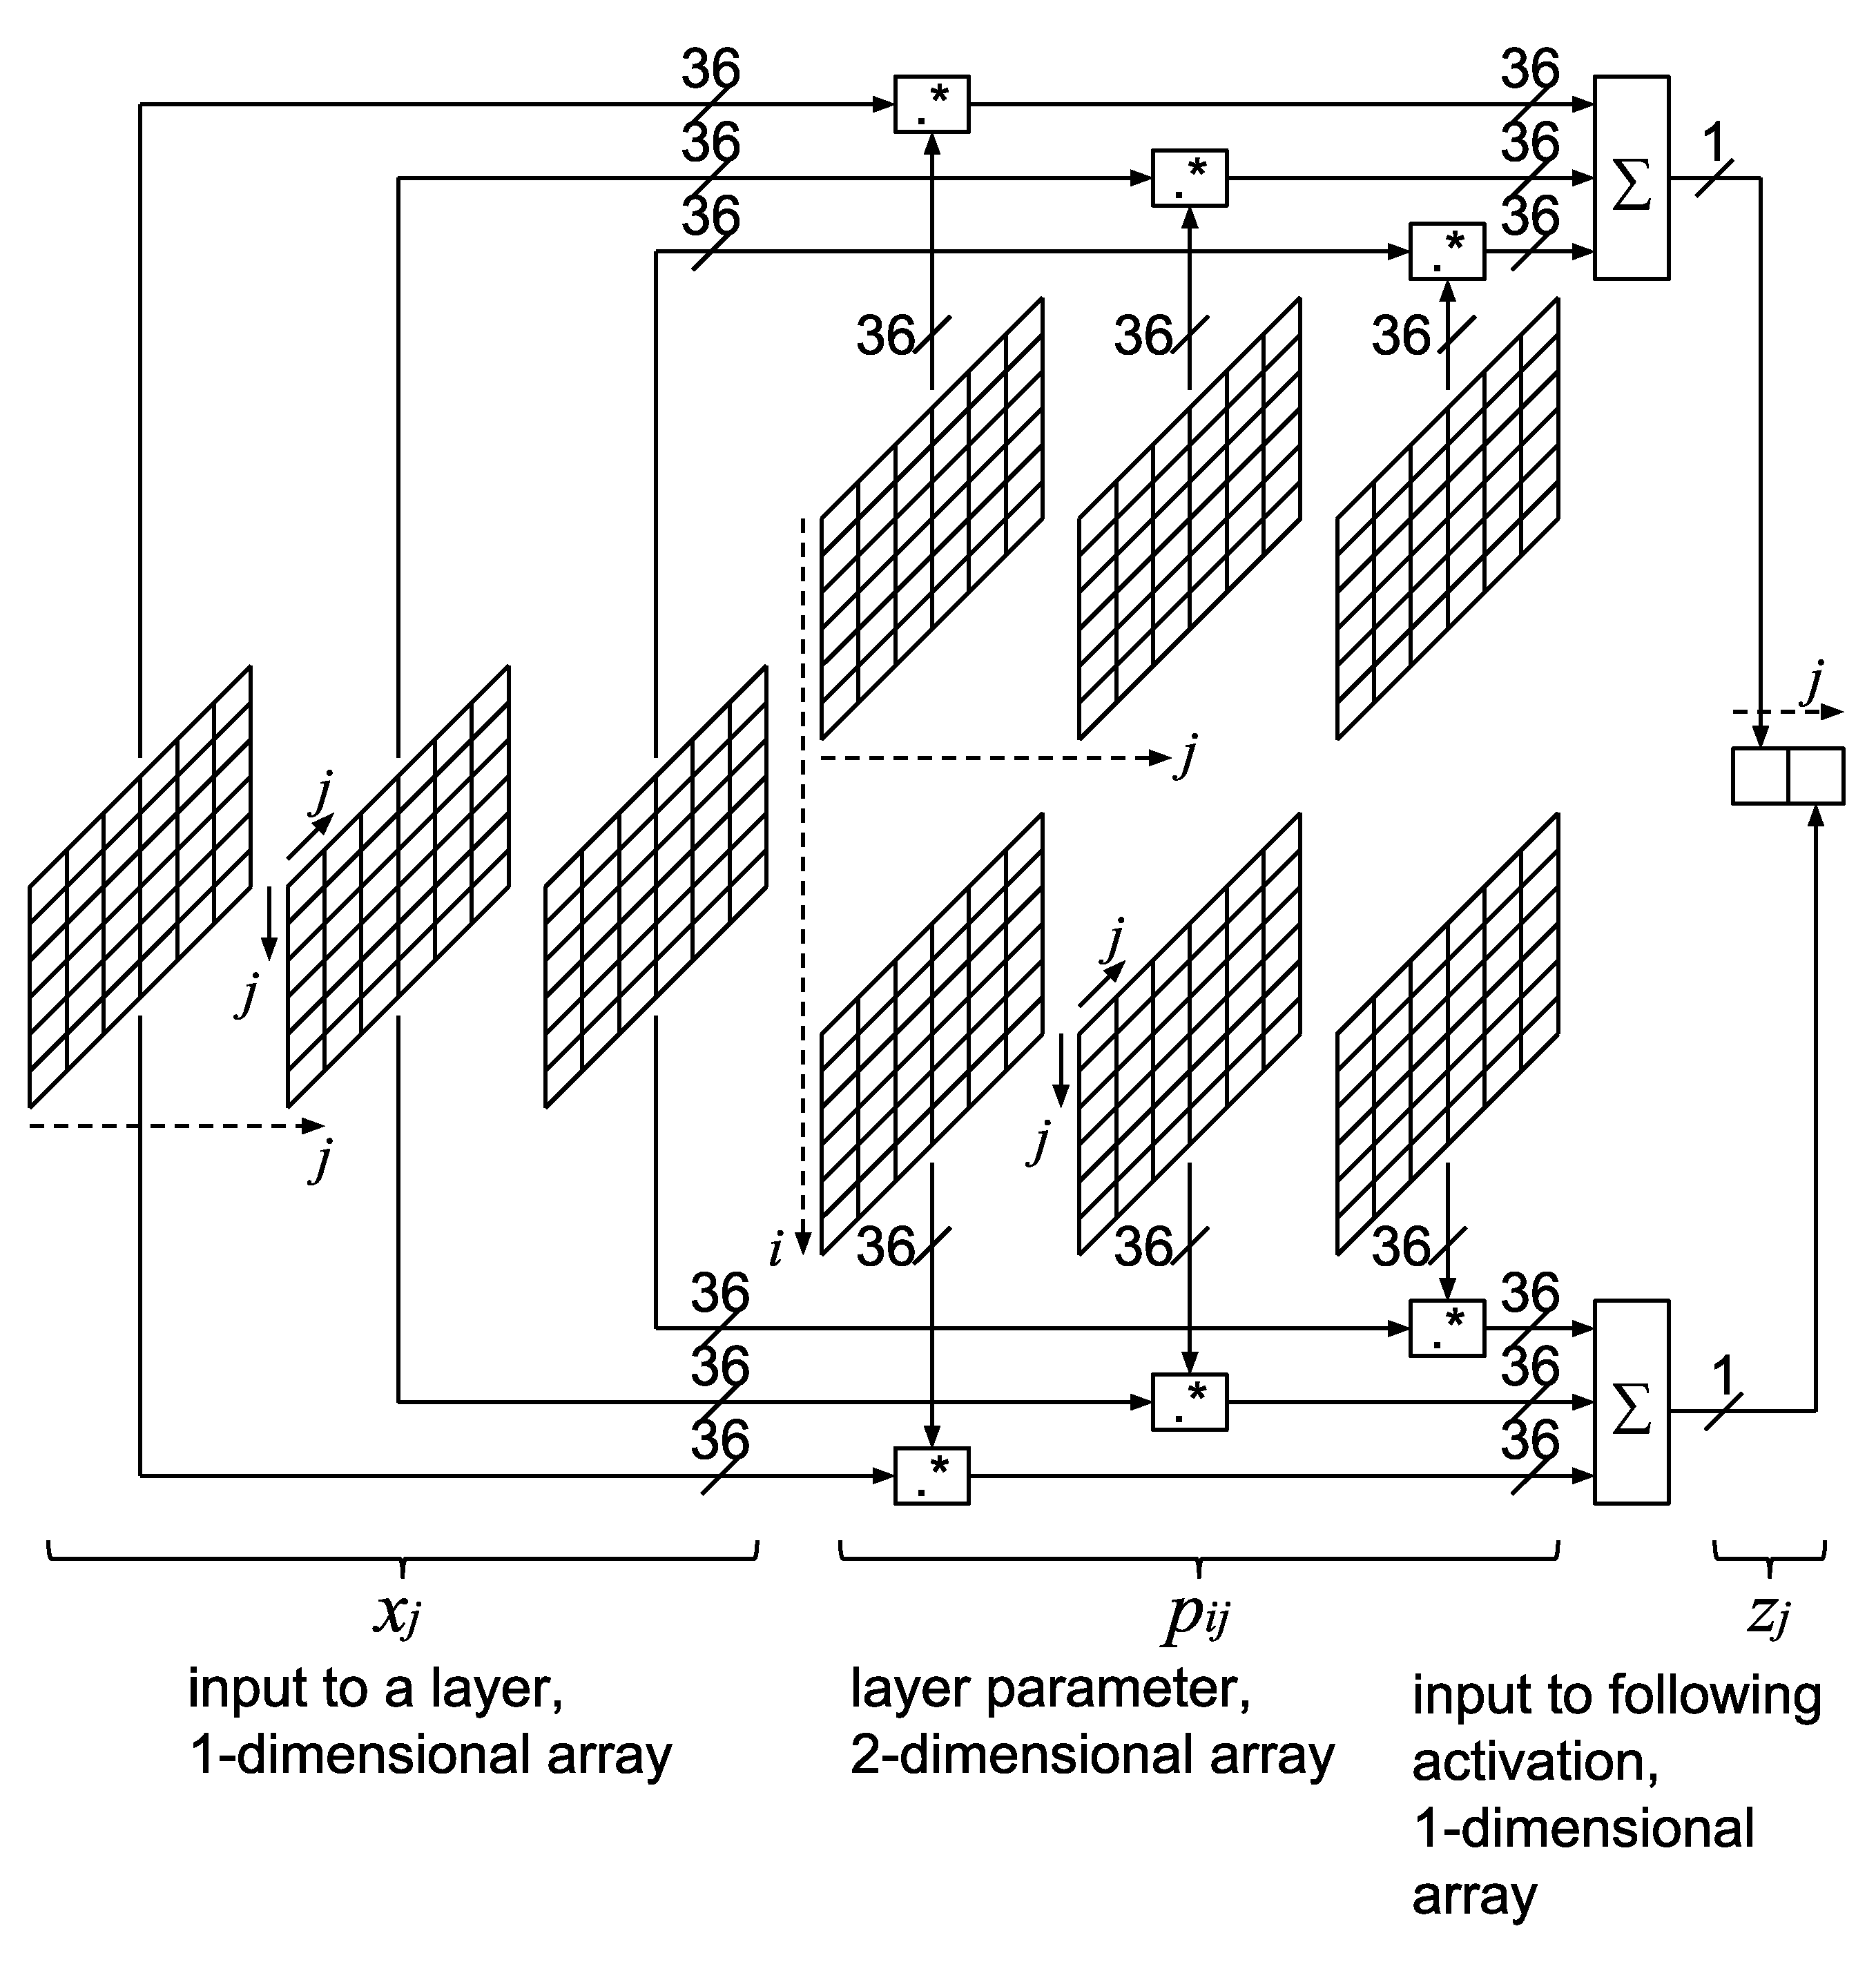
\includegraphics[width=\hsize]{fig/layer_fully_connected_02.eps}
   \caption{fully connected layer}
   \label{fig:layer_fully_connected}
  \end{minipage}
 \end{center}
\end{figure}

\begin{figure}[!tb]
 \begin{center}
  \begin{minipage}{\hsize}
   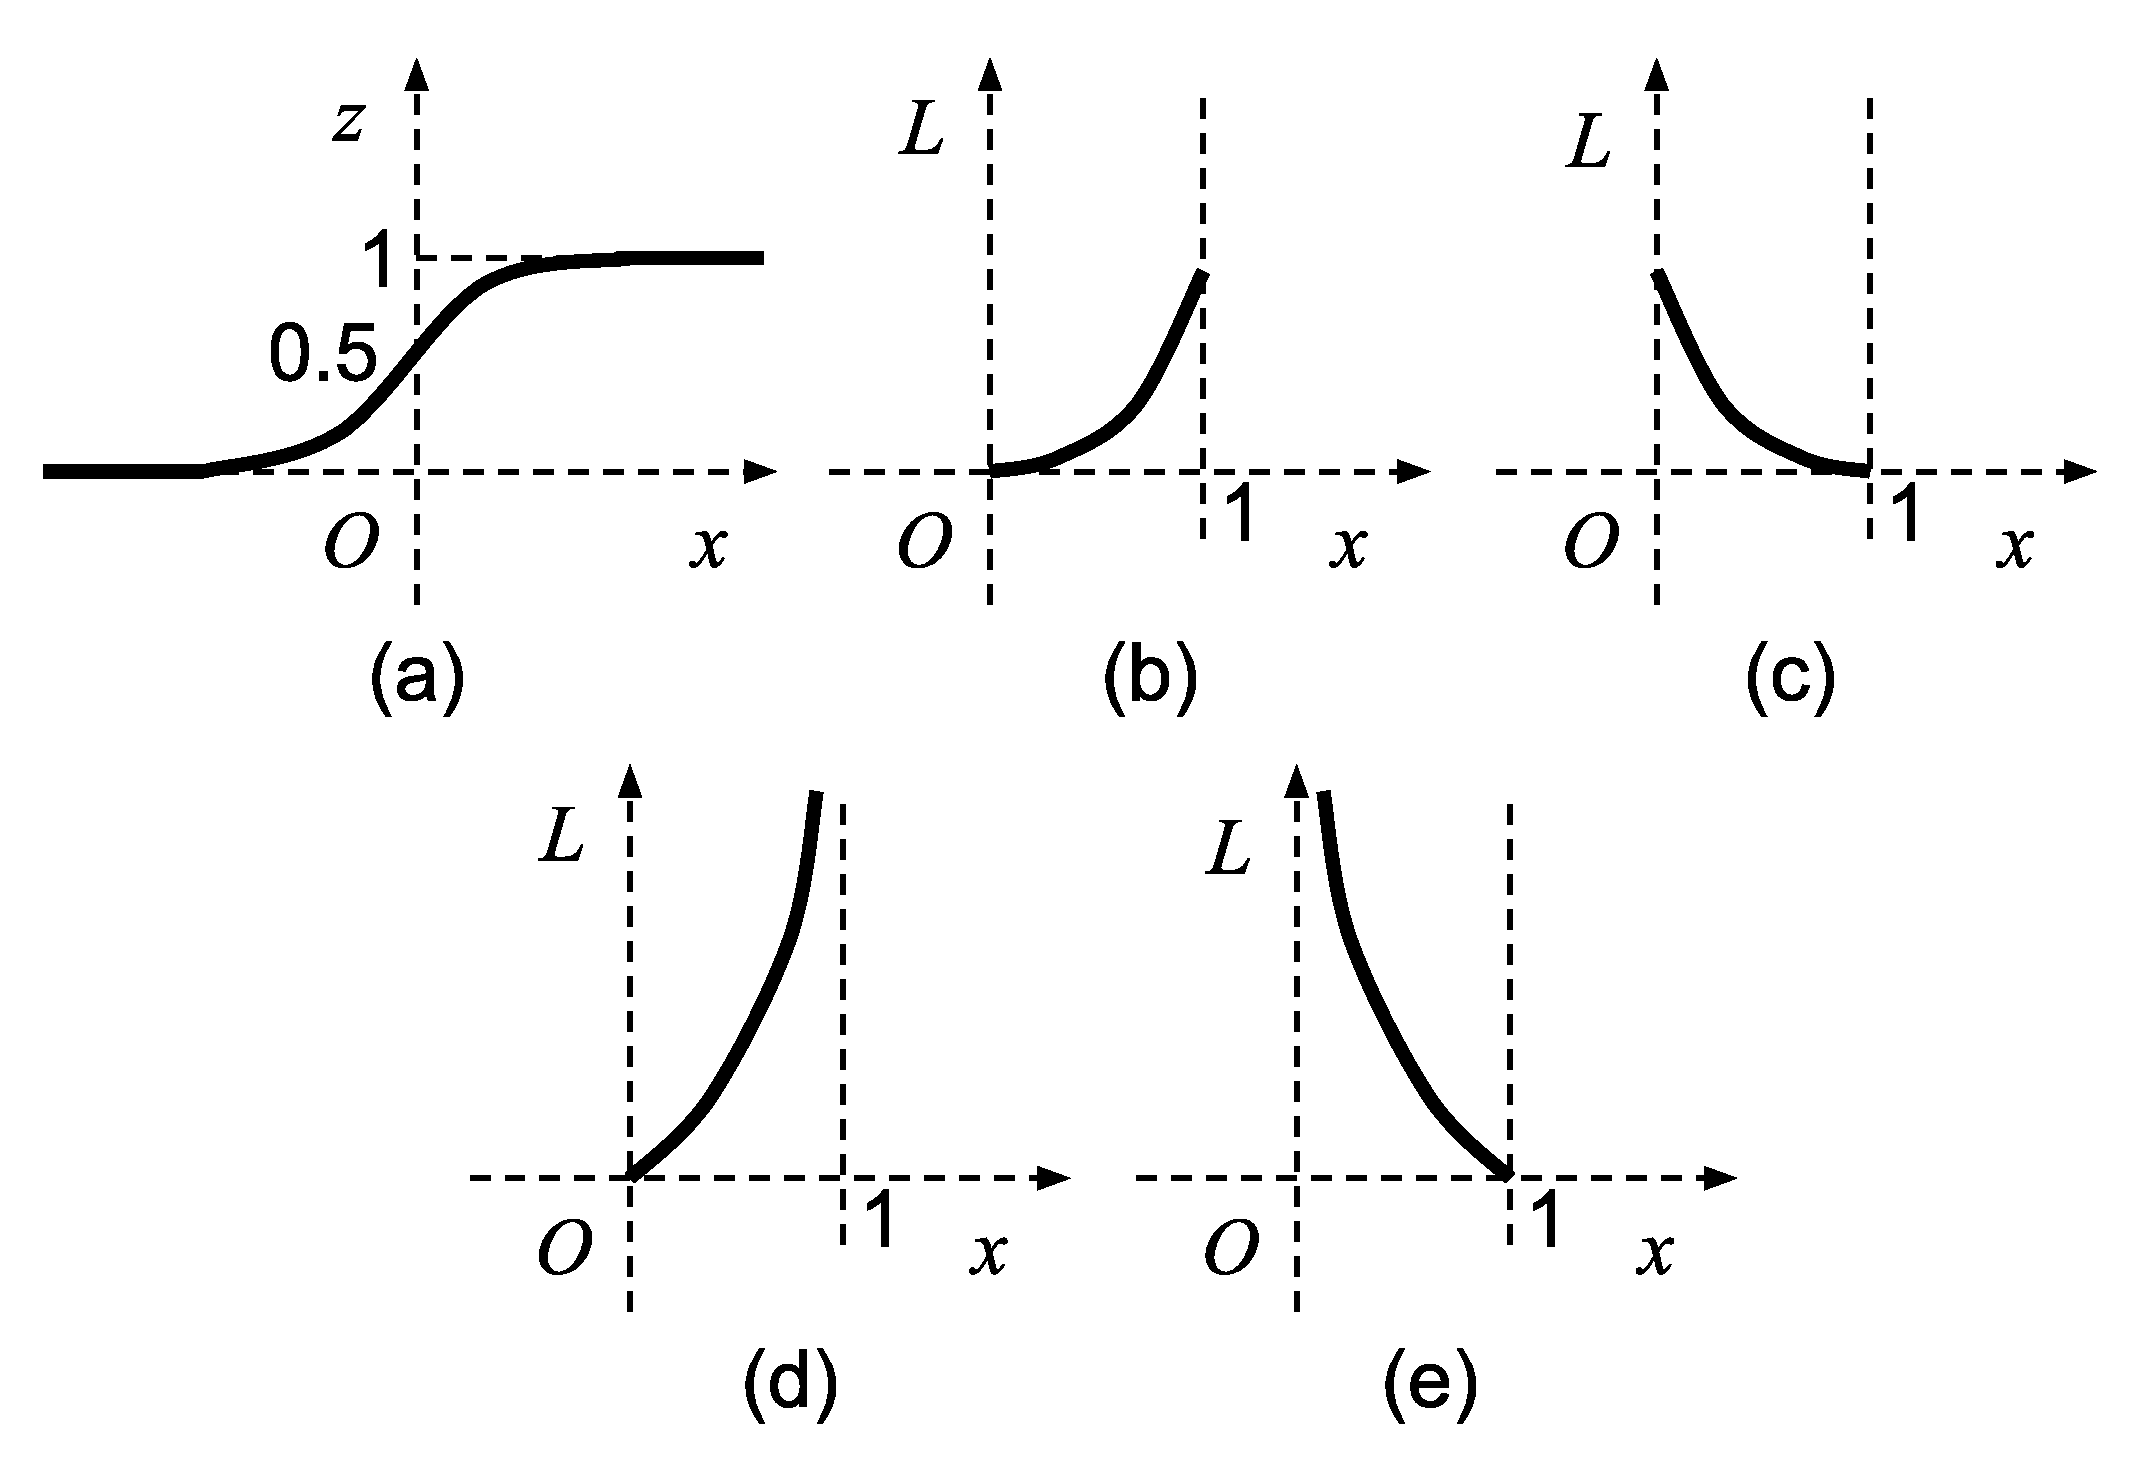
\includegraphics[width=\hsize]{fig/curves_02.eps}
   \caption{(a) sigmoid function
    (b) Euclidean distance when the}
   \label{fig:curves}
  \end{minipage}
 \end{center}
\end{figure}

\begin{figure}[!tp]
 \begin{center}
  \begin{minipage}{\hsize}
   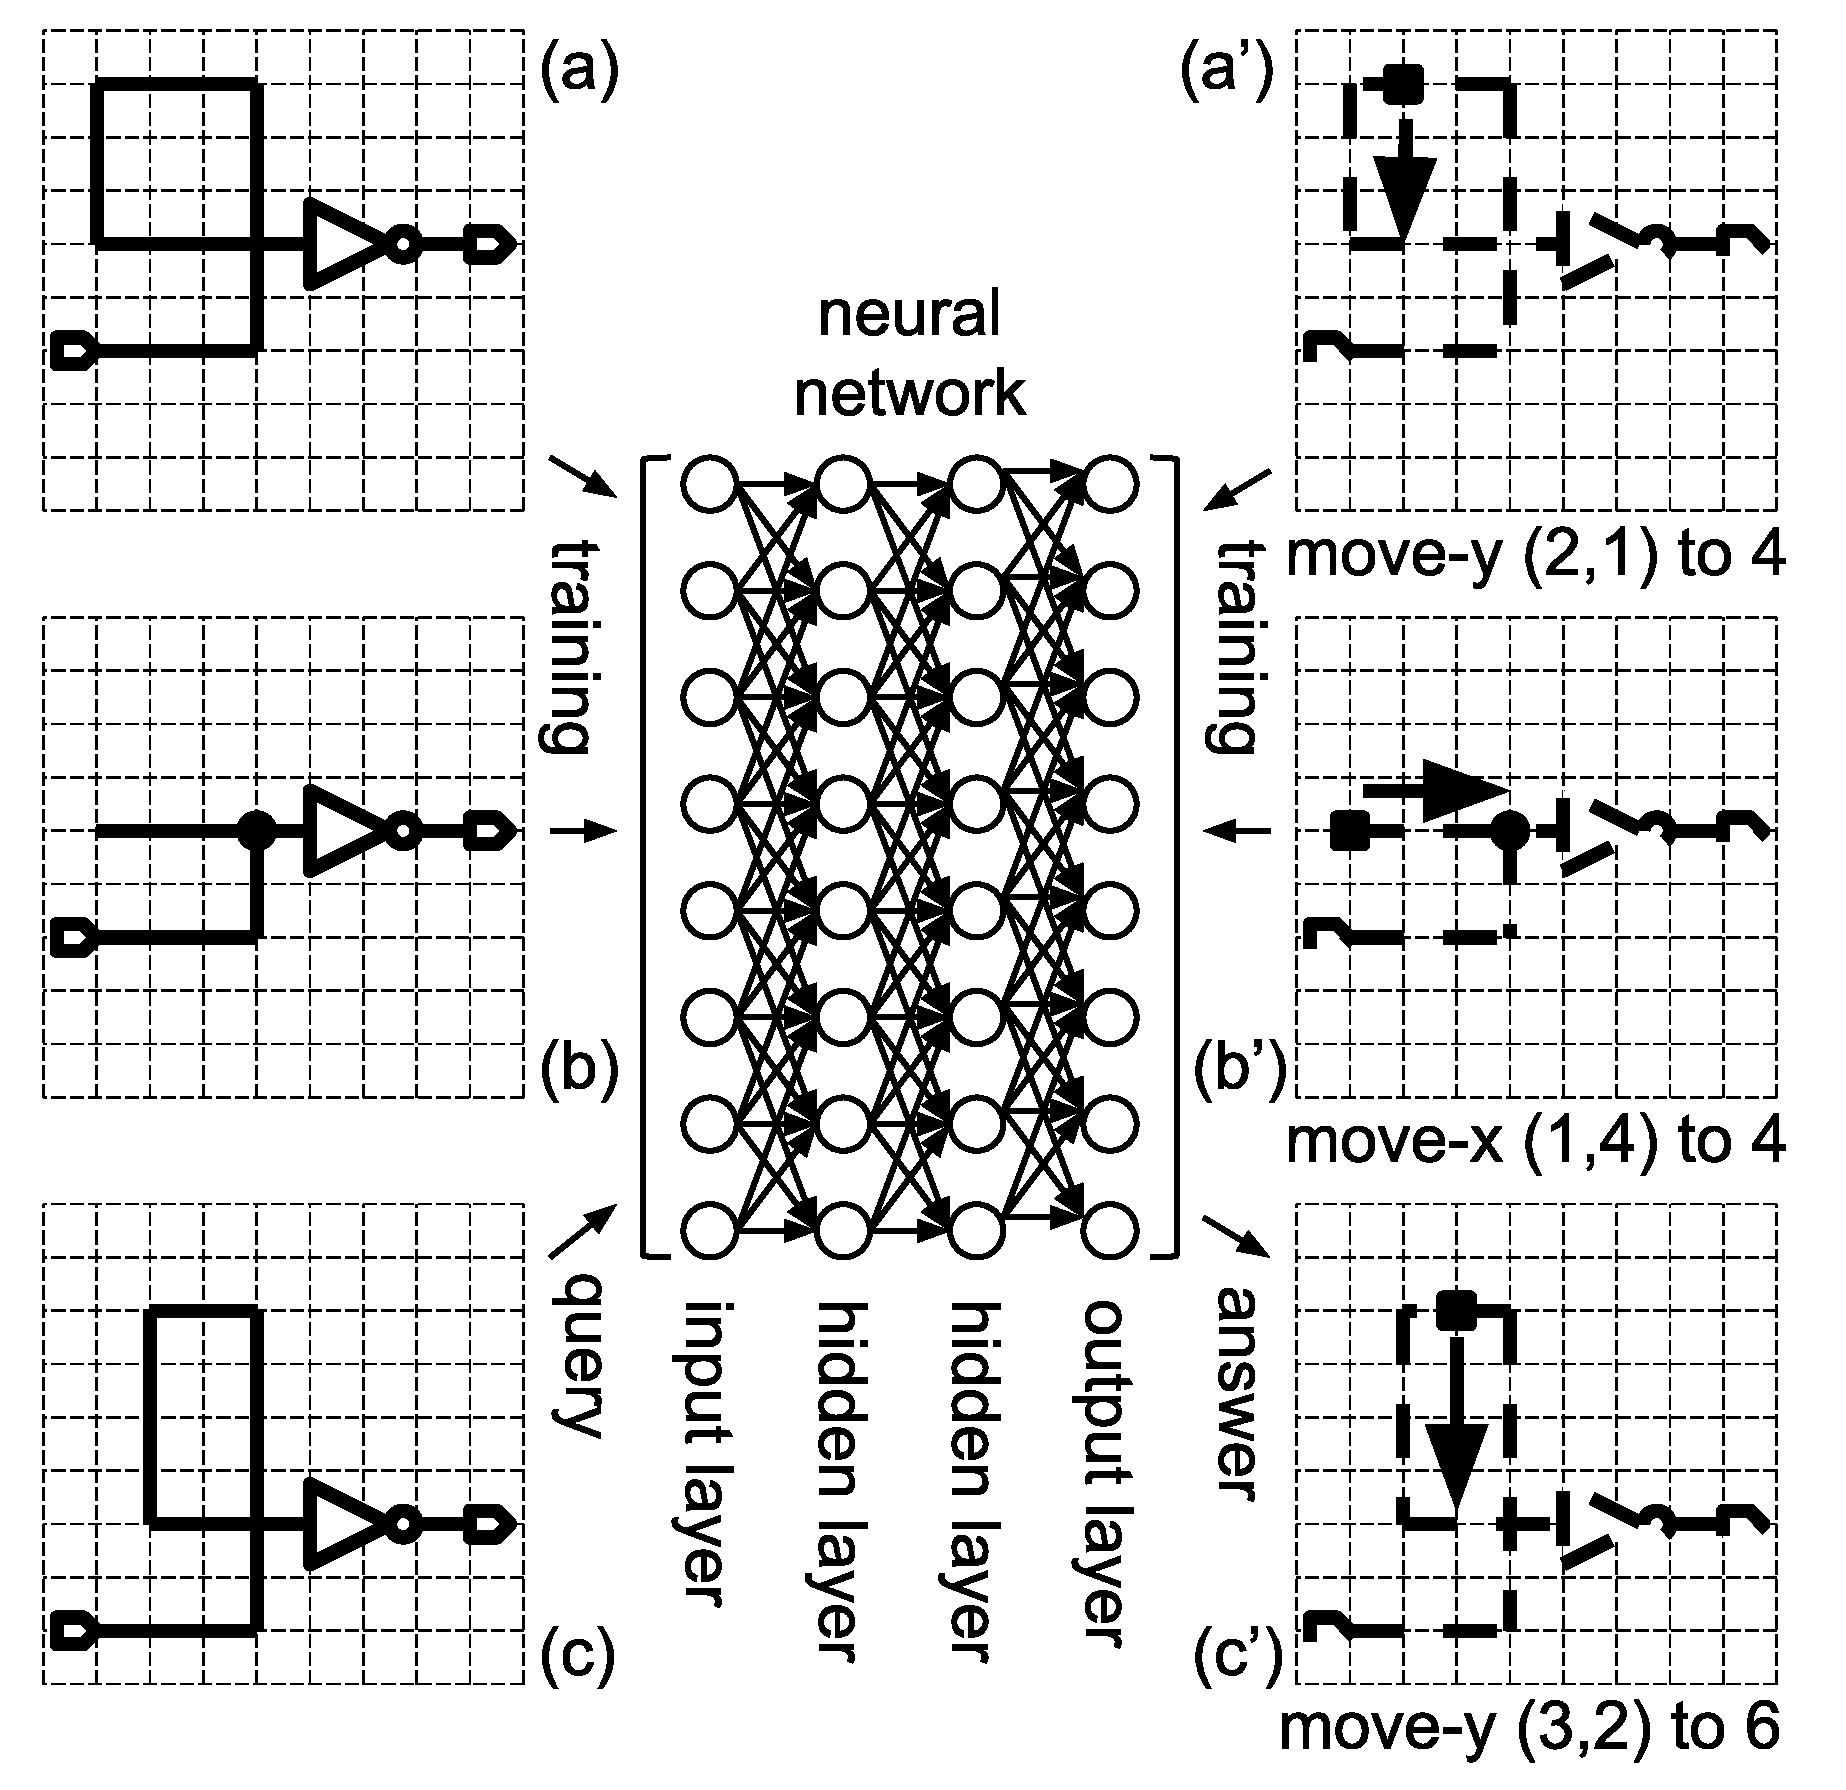
\includegraphics[width=\hsize]{fig/nn_schem_05.eps}
   \caption{training and querying neural network.}
   \label{fig:nn_schem}
  \end{minipage}
 \end{center}
\end{figure}

%Figure {\ref{fig:flow}} shows a concept how to obtain an aesthetic schematic.
%It has a neural network which learns pairs of schematic and editting command
%issued by a human.
%Whichever the schematic is given by a conventional schematic generator
%or other human,
%the trained neural network update the schematic.

Figure \ref{fig:nn_schem} shows a basic concept.
Multilayer neural network described in \cite{mit} is used
to make schematics aesthetic, based on training data created by human.
The input of the neural network is schematic.
The schematics are encoded into 1-dimensional vectors as described later,
so that neural network can accept the schematics.
The output of the neural network is edit command for the schematic.
The edit commands are also encoded into 1-dimensional vector.
Any edit command does not change the semantics of the schematic.
The neural network has parameters to calculate optimal schematic edit command.
The parameters are updated by training.

The command consists of following 4 elements:
\begin{itemize}
\item command, either move-x or move-y
\item origin-x
\item origin-y
\item destination
\end{itemize}
Move-x means to move circuit elements horizontally, as shown (b')
of Fig. \ref{fig:nn_schem}.
Move-y is for vertically moving, as shown (a') and (c')
of Fig. \ref{fig:nn_schem}.
In (a') of Fig. \ref{fig:nn_schem}, 
the command `move-x (2, 1) to 4' can be seen,
where origin-x, origin-y and destination are 2, 1 and 4 respectively.
It means to horizontally move an element at the coordinate (2, 1) to (2, 4).

In Fig. \ref{fig:nn_schem}, (a), (a'), (b) and (b') show training phase.
The neural network parameters are updated by given schematic on input layer
of the nerual network, and given edit command on output side.
It is noted that training data are exposed to output layer
as well as input layer in traning phase,
even though the name is `output layer'.
After traning, the neural network generates schematic edit command
from the output layer
based on its training, as shown (c) and (c') in Fig. \ref{fig:nn_schem}.

\begin{figure}[!tp]
 \begin{center}
  \begin{minipage}{\hsize}
   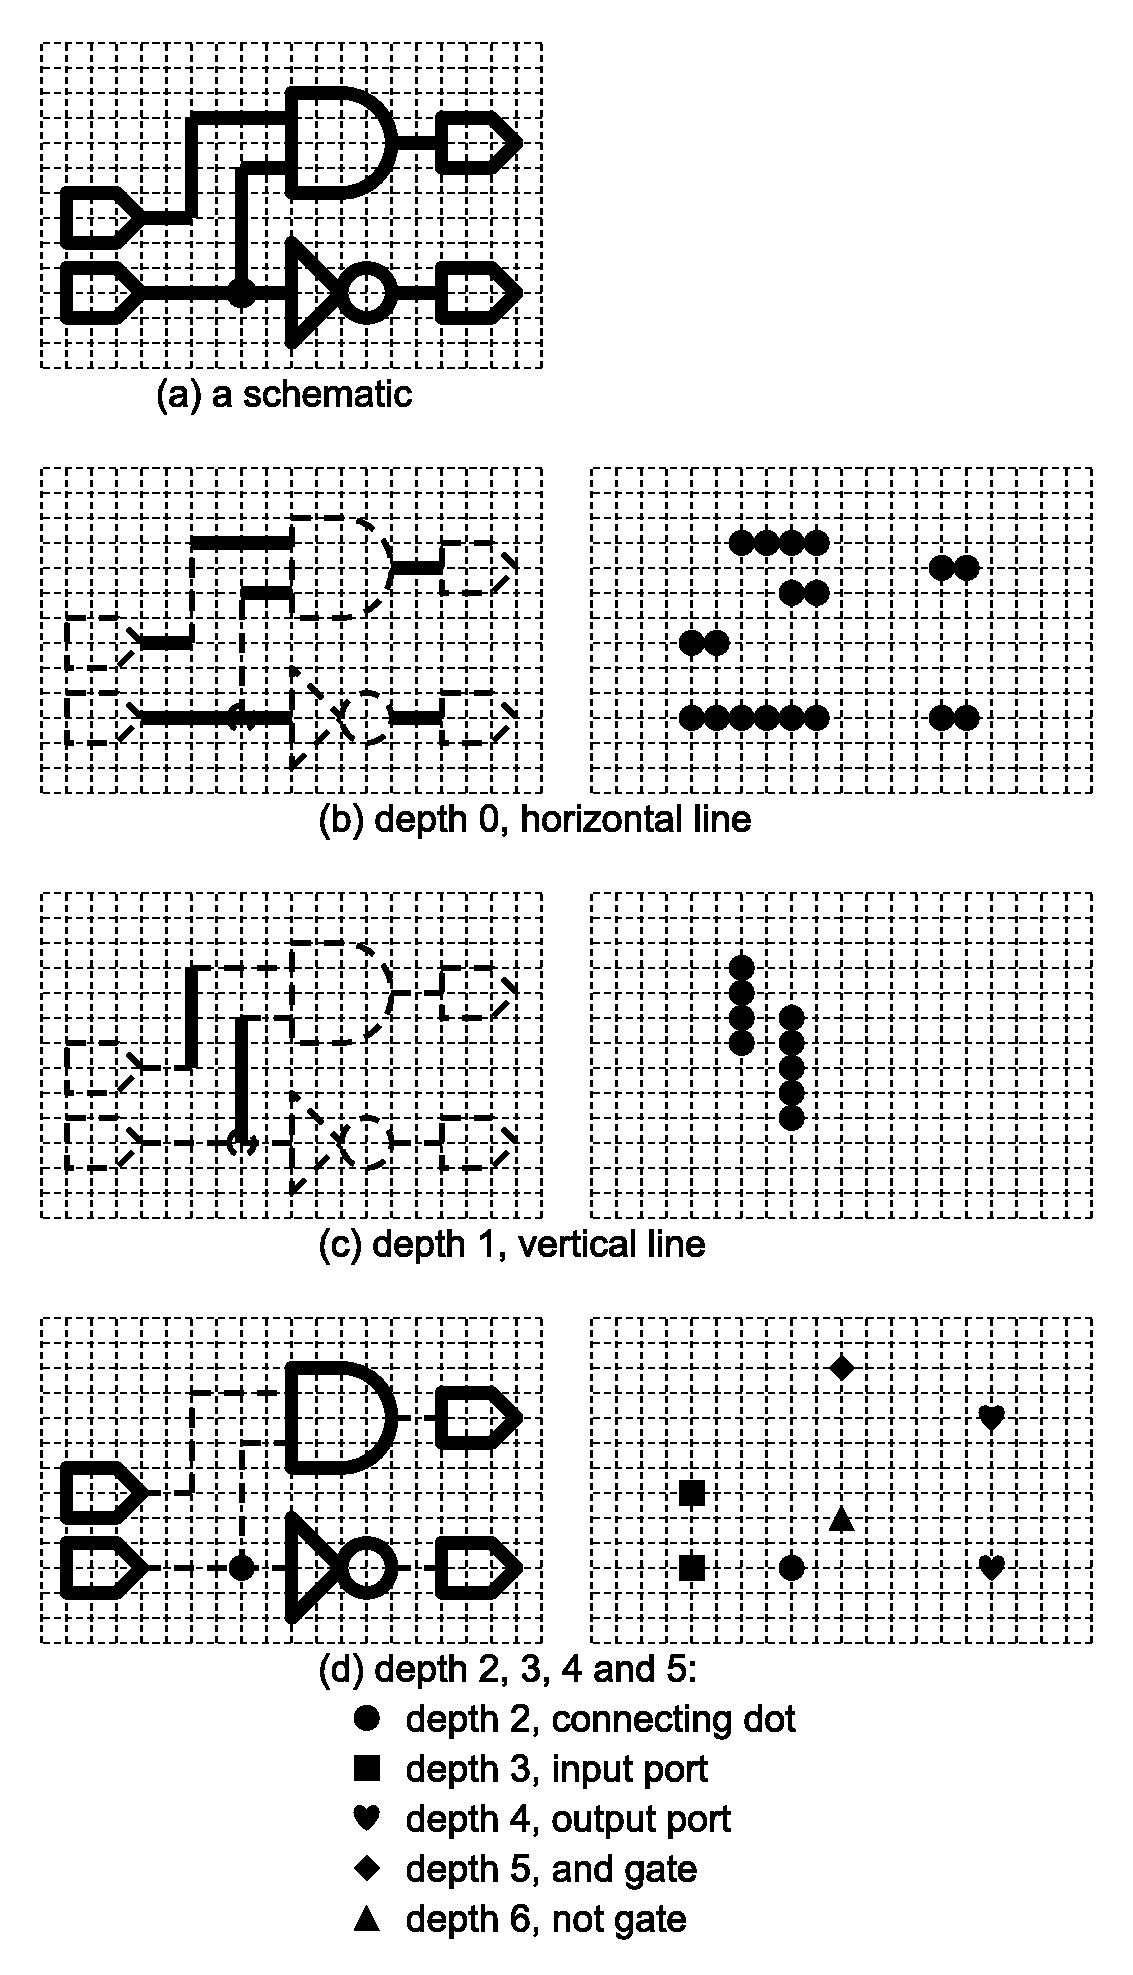
\includegraphics[width=\hsize]{input_encode_03.eps}
   \caption{a way to encode schematic for input vector of neural network}
   \label{fig:input_encode}
  \end{minipage}
 \end{center}
\end{figure}

%To feed schematics and editing command to neural network,
%they are necessary to be encoded into vectors composed of real numbers.
Figure \ref{fig:input_encode} shows the way to encode schematic
for input layer of the neural network.
A 2-dimensional schematic is at first mapped to a 3-dimensional space
where z-axes is type of circuit element, like nets, ports or gates.
After that, a vector is achieved by concatenating the 3-dimensional space
into 1-dimensional vector.

Figure \ref{fig:input_encode} (a) shows a logic schematic composed of
inputs ports, output ports, an and-gate, a not-gate,
horizontal nets, vertical nets, and a connecting point.
Figure \ref{fig:input_encode} (b) picks up horizontal nets appearing
in Fig. \ref{fig:input_encode} (a), and they are mapped to depth 0.
The depth 0 is composed of a 2-dimensional matrix which size is the same
as given schematic.
In the right side of (b) in Fig. \ref{fig:input_encode},
dots are located at coordinates where horizontal nets appear.
Points with dots corresponds to a value of 1.0, ones without dots
corrensponds to a value of 0.0.
As shown in figure \ref{fig:input_encode} (c),
vertical nets are mapped to depth 1.
As well, connecting dots, input ports, output ports, and-gates and not-gates
are mapped to depth 2, 3, 4, 5 and 6, respectively.
Input vectors are finally obtained by flattening the multi-layer of matrices.

\begin{figure}[!tp]
 \begin{center}
  \begin{minipage}{\hsize}
   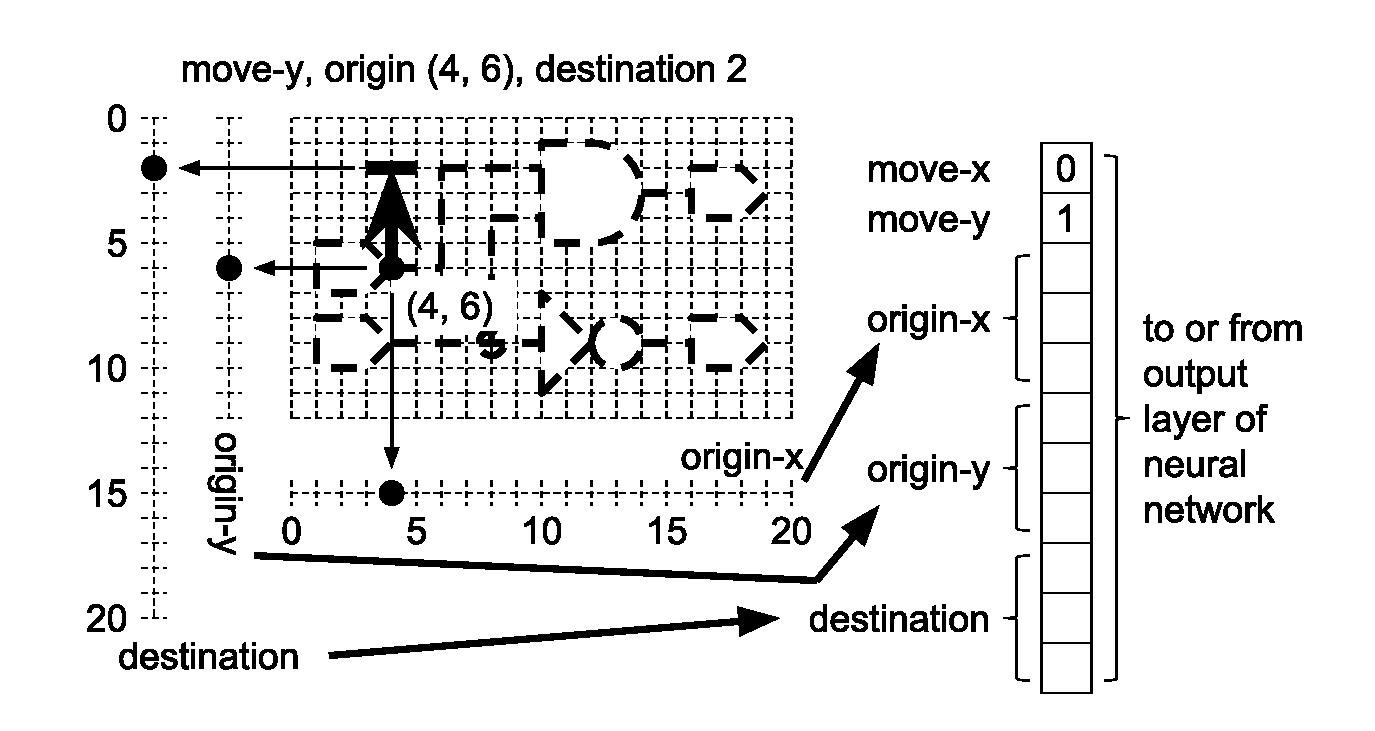
\includegraphics[width=\hsize]{output_encode_02.eps}
   \caption{a way to encode edit commands for output vector of neural network}
   \label{fig:output_encode}
  \end{minipage}
 \end{center}
\end{figure}

Figure \ref{fig:output_encode} shows a way to encode editing commands
for output vector of the neural network.
%A command `move-y, origin (4, 6), destination 2' is shown in the figure
%as an example, which means to vertically move a object at the point (4, 6)
%to y-coordinate of 2.
%The more general explanation of editing commands follow.
%Editing command consist of three elements.
%The first element is a type of command.
%Only 2 kinds of commands are used in this paper,
%which are move-x and move-y,
%although the other commands could be introduced as long as
%the command would not change the semantics of the schematic.
%Move-x means to move a object horizontally.
%Move-y means to move one vertically.
%The second element is a 2-element vector, meaning origin of the command.
%The vector consists of x and y coordinates of the origin.
%The third element is destination.
%The destination means x-coordinate when the type of command
%is move-x, in this work.
%It becomes y-coordinates when the command if move-y.
Move-x is encoded to the vector $[1.0, 0.0]$, 
while move-y is encoded to the vector $[0.0, 0.1]$. 
Origin-x is encoded to one-hot vector, which is
\begin{itemize}
\item $[1.0, 0.0, 0.0, 0.0, \cdots]$ for 0,
\item $[0.0, 1.0, 0.0, 0.0, \cdots]$ for 1, 
\item $[0.0, 0.0, 1.0, 0.0, \cdots]$ for 2,
\end{itemize}
and so on.
For origin-x, the length of the one-hot is the width of the schematic.
The y coordinate is also encoded to one-hot vector which length is
height of the schematic.
As well, destination is one-hot vector which length is
maximum value of width and height of the schematic.
Output vector of the neural network is eventually obtained
by concatenating those 4 one-hot vectors.

\section{Condition of Experiment}

\begin{figure*}[!tp]
 \begin{center}
  \begin{minipage}{\hsize}
   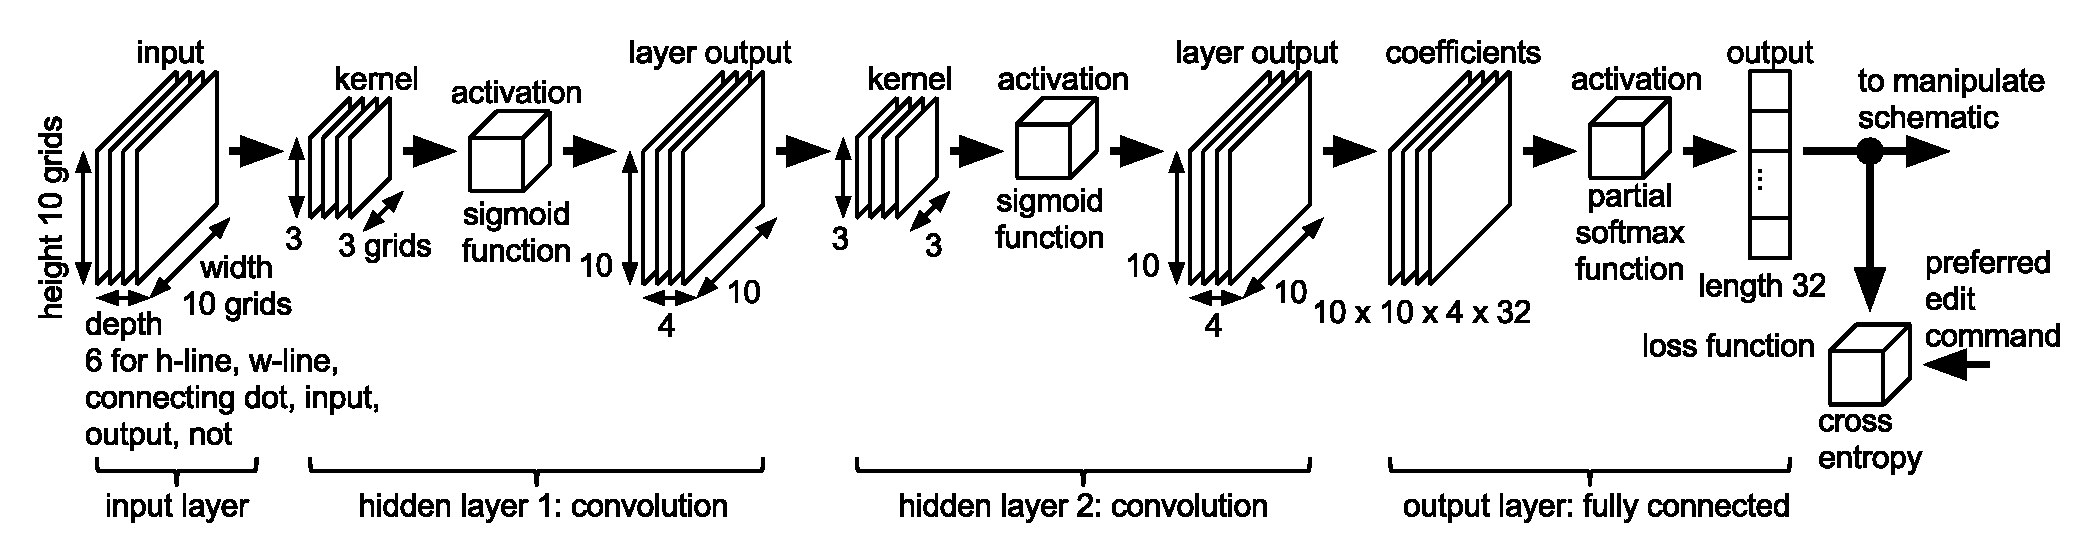
\includegraphics[width=\hsize]{fig/layers_05.eps}
   \caption{a layer structure of the neural network}
   \label{fig:layers}
  \end{minipage}
 \end{center}
\end{figure*}

\begin{figure}[!tp]
 \begin{center}
  \begin{minipage}{\hsize}
   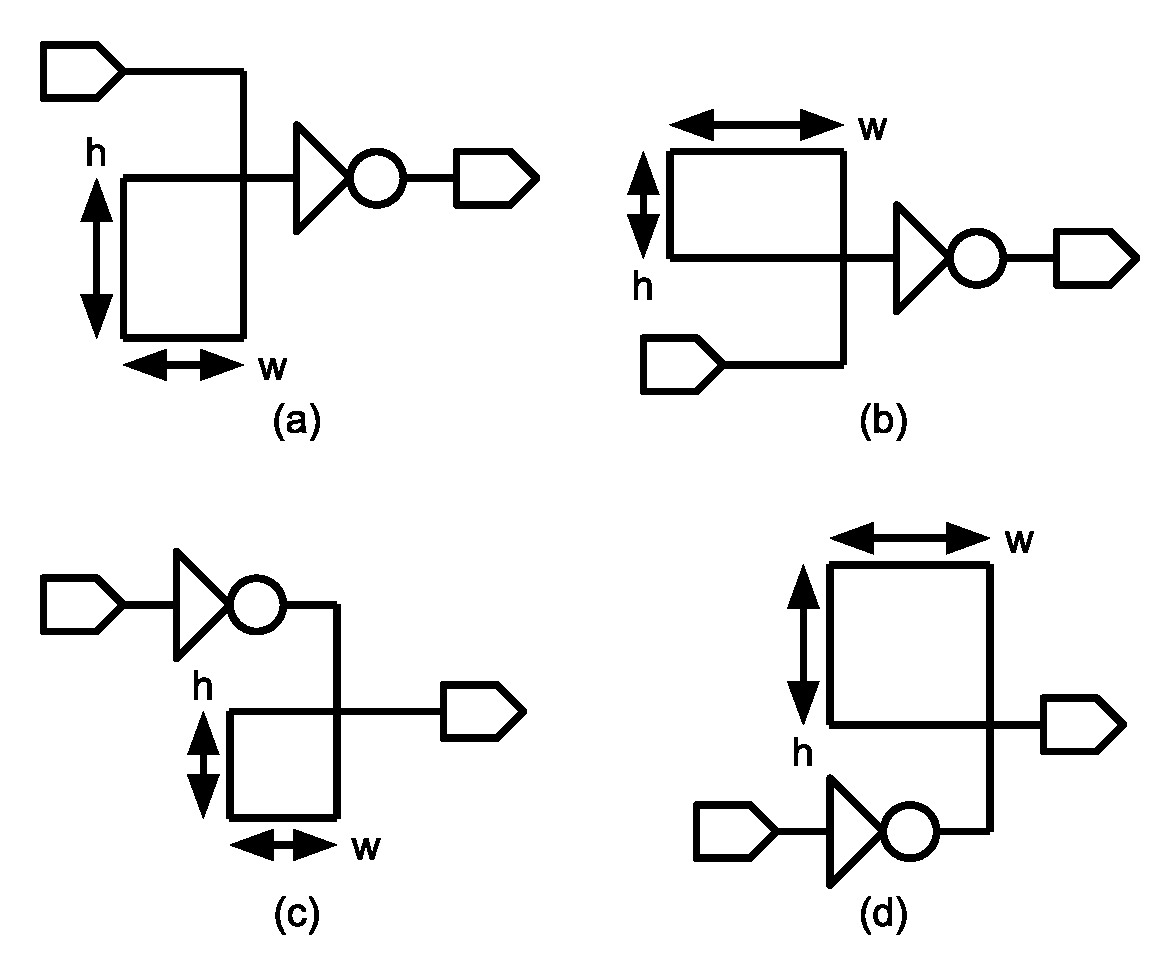
\includegraphics[width=\hsize]{fig/training_data_01.eps}
   \caption{training data}
   \label{fig:training_data}
  \end{minipage}
 \end{center}
\end{figure}

Schematics shown in Fig. \ref{fig:training_data} are used for this experiments.
Each one contains one input port, one not gate and one output port.
It also contains an unnecessary ring which will be removed
by the edit commands generated by the trained neural network.
Each schematic has 9 variations with
$w$ of 2, 3 and 4, for the widht of the ring,
$h$ of 2, 3 and 4, for the height of the ring.
So $9 \times 4 = 36$ different schematic patterns are introduced.
The schematic dimension is 10 grids $\times$ 10 grids.
There is margin around the schematics,
so the schematics can be placed various position on schematic field.
Finally, several steps are introduced to achieve a clean schematics.
The total numbers of schematic-edit-command pairs amounts up to about 1000.

Figure \ref{fig:layers} shows a layer structure of neural network.
The input layer has width of 10, height of 10,
depth of 6 for horizontal net, vertical net, connecting dot, input port,
output port and not gate.
The first hidden layer is a convolutional layer \cite{mit},
where kernel dimension is $3\times 3$, output depth is 4.
The first hidden layer is activated by sigmoid function.
The second hidden layer is another convolutional layer,
where kernel dimension is $3\times 3$, output depth is 4,
activated by sigmoid function.
The output layer is a dense layer.
The input vector size of the output layer
is detemined by product of schematic dimension
and output length of previous layer, which is $10 \times 10 \times 4$.
The output length of the layer is sum of 2 for command type,
10 for origin-x, 10 for origin-y and 10 for destination.

The following hyper-parameters are used:
0.1 for learning rate, 16 for minibatch size, 10000 of traning iteration.
The program is written in Java and Clojure,
a Lisp dialect running of Java Virtual Machine.

\begin{figure}[!tp]
 \begin{center}
  \begin{minipage}{\hsize}
   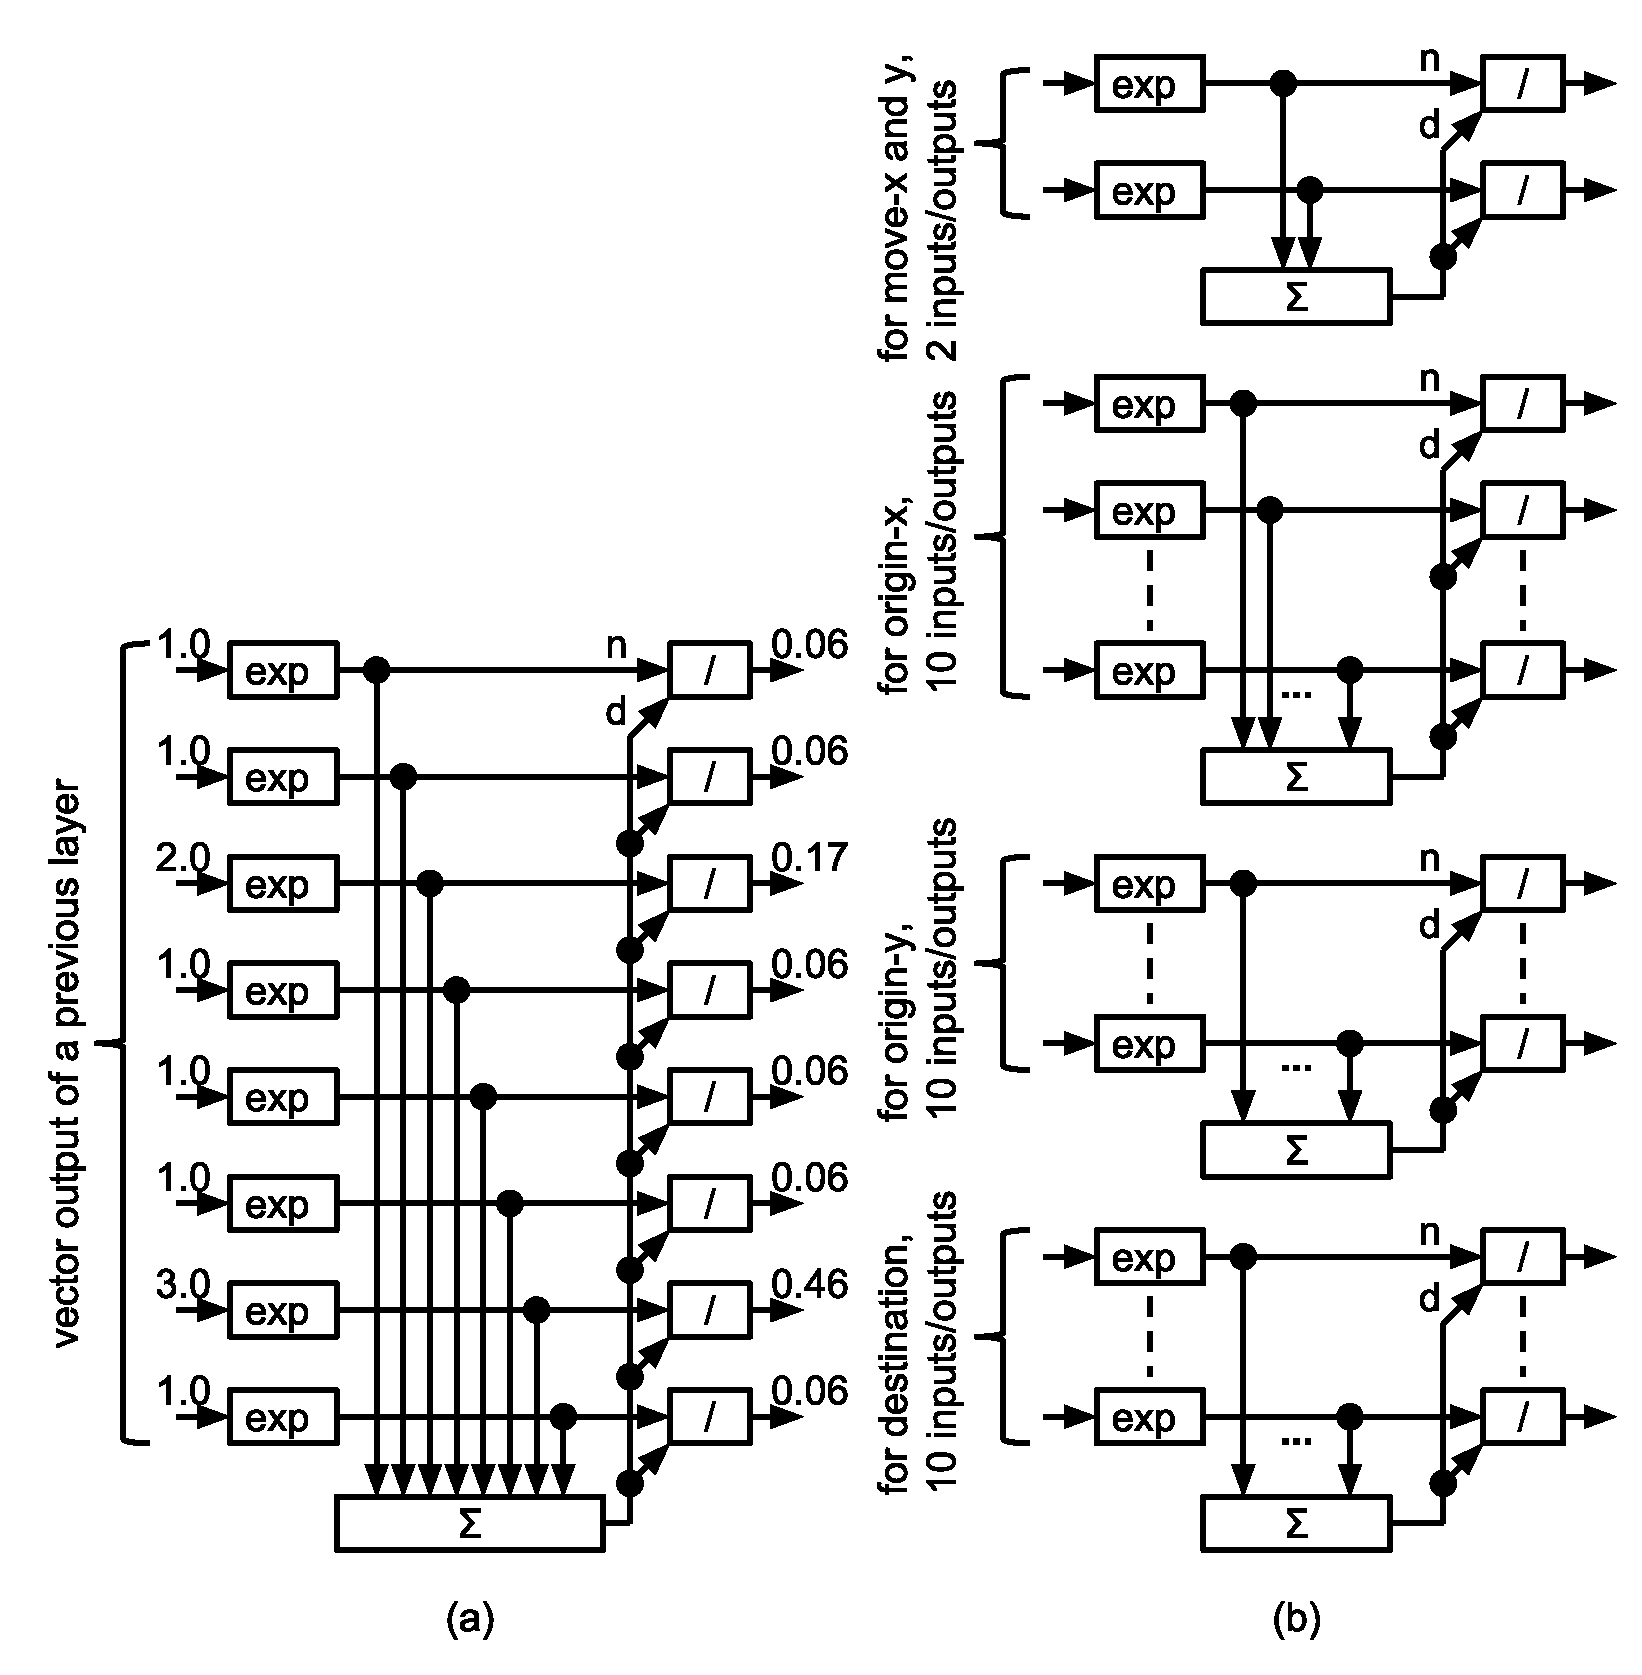
\includegraphics[width=\hsize]{fig/partial_softmax_05.eps}
   \caption{(a) conventional softmax, (b) partial softmax used in this work.}
   \label{fig:partial_softmax}
  \end{minipage}
 \end{center}
\end{figure}

The output layer is activated by softmax function.
The (a) of Fig. \ref{fig:partial_softmax} shows a conventional softmax
function shown in \cite{mit}.
It emphasizes the maximum value in the input vector,
by dividing exponential function of each input by the sum of those.
Softmax function is introduced to pickup one element of vector.
In this study, it is not suitable to pick up only one element
amoung mixture of command type, origin-x, origin-y and destination.
but is preferable to pick up them from each part of the vector independently.
Then the partial softmax shown in (b) of Fig. \ref{fig:partial_softmax}
is used where softmax function is applied
for the first 2 elements for command type,
the next 10 elements for origin-x, 10 for origin-y and last 10 for destination.

\section{Result}

\begin{figure}[!tp]
 \begin{center}
  \begin{minipage}{\hsize}
   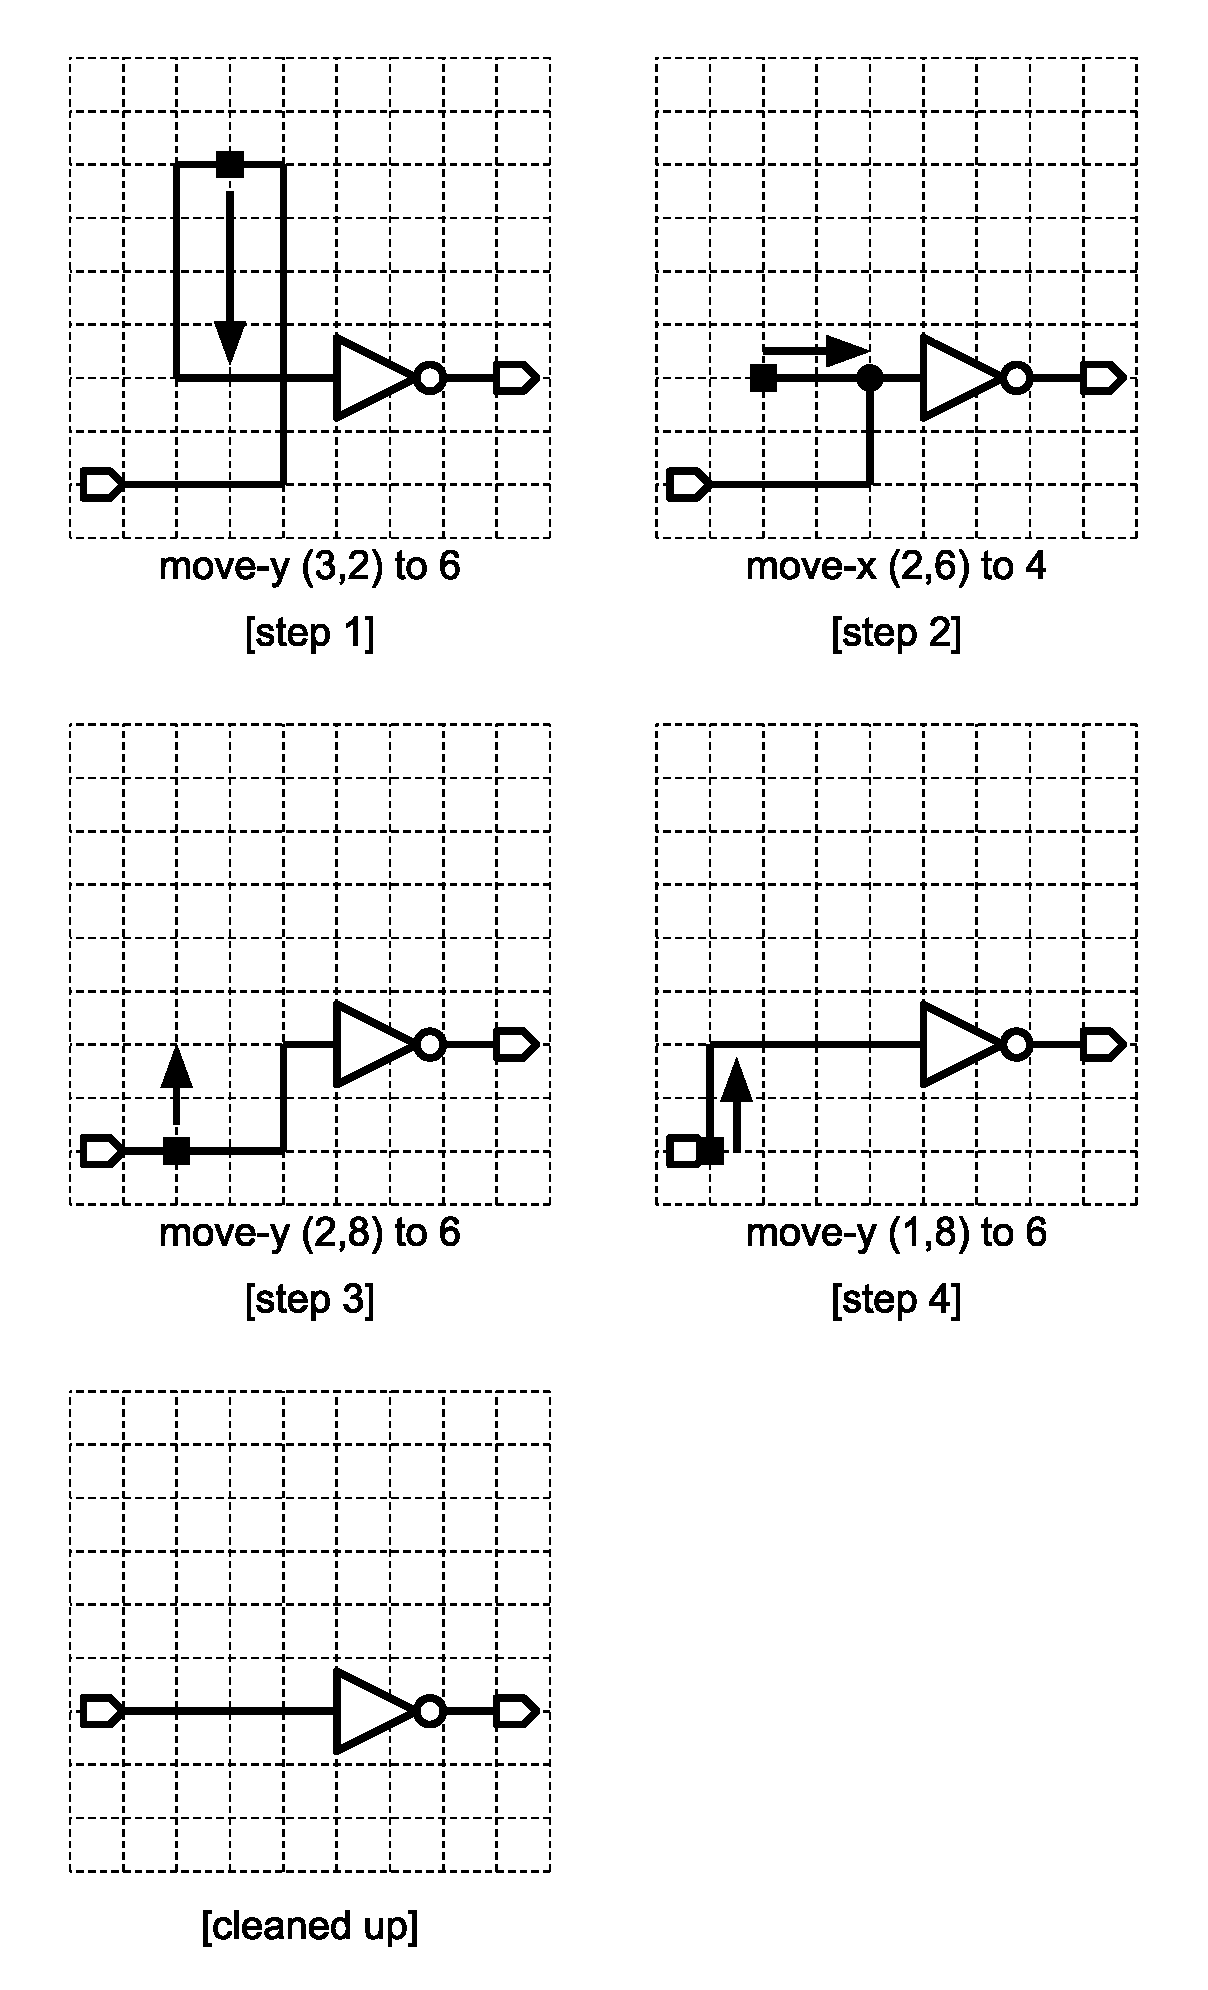
\includegraphics[width=\hsize]{fig/edit_steps_02.eps}
   \caption{steps to make the schematic aesthetic by trained neural network.}
   \label{fig:edit_steps}
  \end{minipage}
 \end{center}
\end{figure}

Figure \ref{fig:edit_steps} shows steps of circuit edit
automatically generated from the trained neural network.
For this result, 12 schematic patterns are used for traning
out of 36 patterns shown in Fig. \ref{fig:training_data}.
A schematic unused for traning is picked up,
then challenged by the tranined neural network.
In Fig. \ref{fig:edit_steps}, filled square shows the origin-x and y
for each step.
At step 1, the top net of the unnecessary ring is grabbed and moved lower
to remove the ring.
At step 2, the edge of salient net is grabbed,
and moved to the adjacent cross point.
At step 3, the net connected to the input port is grabbed .
Finally, at step 4, the input port is moved upward
and a clean schematic is achived.
The neural network succeeded in clean up a schematic
which the network has never experienced.

\begin{figure}[!tp]
 \begin{center}
  \begin{minipage}{\hsize}
   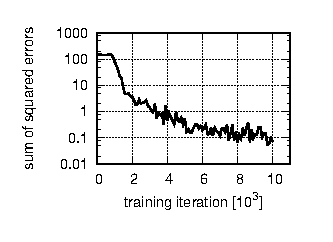
\includegraphics[width=\hsize]{fig/errors.eps}
   \caption{convergence of error}
   \label{fig:errors}
  \end{minipage}
 \end{center}
\end{figure}

Figure \ref{fig:errors} shows a error appearing learning phase.
The horizontal axes is traning iteration up to 10000.
The vertical axes is the sum of squared errors between
neural network output and training data for output layer.
Convergence can be seen there.
It takes 60 seconds to finish 10000 training iterations.

\begin{figure}[!tp]
 \begin{center}
  \begin{minipage}{\hsize}
   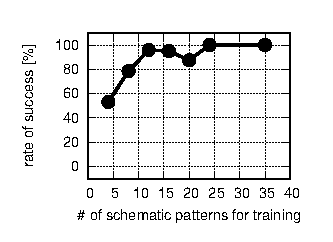
\includegraphics[width=\hsize]{fig/test_data.eps}
   \caption{rate of success of revising the schematics}
   \label{fig:test_data}
  \end{minipage}
 \end{center}
\end{figure}

This experiment has been performed varing the number of schematic patterns.
Figure \ref{fig:test_data} shows the result.
The horizontal axes shows the number of schematic patterns used for traninig
out of 36 patterns in total.
Patterns not in the traning data are challeged to be cleaned up.
The vertical axes shows the rate of success.
Success means that a clean schematic
without a overcrossing or unnecessary corner is achived
like the bottom subfigure of Fig. \ref{fig:edit_steps}.
Even when trained with only 4 patterns,
the neural network can clean up about 50\% of schematic.
When trained with 12 patterns,
which corresponds to one third of all schematic patterns,
the rate of success exceeds 90\%.
When trained with 24 patterns,
which corresponds to two thirds of all schematic patterns,
the rate reached to 100\%.


\section{Conclusions}

An novel way to achieve aesthetic schematic is proposed.
Deep neural network is used, and it learns how to edit schematic
from edit history obtained from human.
The trained neural network cleans up unnecessary part of given schematics,
which the neural network has not experienced.
Even the neural network is short of traning data,
it can clean up unknown schematics to a certain extent.
With enough training data,
the trained neural network can clean up almost of schematic.

%this is how to do an unnumbered subsection 
%\section*{\sc Acknowledgements}
%This article was written by referring to {\em ``Author's guide --
%Preparation of Papers in Two-Column Format for VLSI Symposia on
%Technology and Circuits''}, the {\em ``Preparation of Papers in
%Two-Column Format for the Proceedings of the 32nd ACM/IEEE Design
%Automation Conference''} written by Ann Burgmeyer, IEEE and {\em ``the
%template for producing IEEE-format articles using \LaTeX''}, written by
%Matthew Ward, Worcester Polytechnic Institute.

\begin{thebibliography}{99}
\footnotesize

\bibitem{ph}
D. A. Patterson, and J. L. Hennessy,
{\em Computer Organization and Design MIPS Edition:
 The Herdware/Software Interface,}
Morgan Kaufmann, 2013.

\bibitem{nauts}
C. Nauts,
``Creating a nice-looking schematic from its netlist description,''
in {\em Proc. Euro ASIC}, Mar. 1992.

\bibitem{anshul}
A. Kumar, A, Arya, V. V. Swaminathan, and A. Misra,
``Automatic Generation of Digital System Schematic Diagrams,''
{\em IEEE Design \& Test of Computers,}
vol. 3, pp. 58--65, 1986.

\bibitem{fiduccia}
C. M. Fiduccia, and R. M. Mattheyses,
``A Linear-Time Heuristic for Improving Network Partitions,''
in {\em Proc. IEEE/ACM Design Automation Conference(DAC),}
Jun. 1982.

\bibitem{chun}
R. K. Chun, K.-J. Chang, and L. P. McNamee,
``VISION: VHDL Induced Schematic Imaging on Net-Lists,''
in {\em Proc. IEEE/ACM Design Automation Conference(DAC),}
Jun. 1987.

\bibitem{green}
L. D. Green, and J. Andersen,
``Automated generation of analog schematic diagrams,''
in {\em Proc. IEEE International Symposium on Circuits and Systems(ISCAS),}
May. 1990.

\bibitem{tsung}
T. D. Lee, and L. Pl. McNamee,
``Aesthetic Routing for Transistor Schematics,''
in {\em Proc. IEEE/ACM International Conference
 on Computer-Aided Design(ICCAD),}
Nov. 1992.

\bibitem{bogdan}
B. G. Arsintescu,
``A Method for Analog Circuits Visualization,''
in {\em Proc. International Conference on Computer Design (ICCD),}
Oct. 1996.

\bibitem{fan}
F. Lin, and K.-T. Cheng,
``An Artificial Neural Network Approach for Screening Test Escapes,''
in {\em Proc. Asia and South Pacific Design Automation Conference (ASP-DAC),}
Jan. 2017.

\bibitem{sourav}
S. Das, J. R. Doppa, D. H. Kim. P. P. Pande, and K. Chakrabarty,
``Optimizing 3D NoC design for energy efficiency:
 A machine learning approach,''
in {\em Proc. IEEE/ACM International Conference on
 Computer-Aided Design (ICCAD),}
Nov. 2015.

\bibitem{nips}
A. Krezhevsky, I. Sutskever, and G. E. Hinton,
``ImageNet Classification with Deep Convolutional Neural Networks,’’
in {\em Proc. Annual Conference on Neural Information Processing Systems (NIPS)},
Dec. 2012.


\bibitem{alphago}
D. Silver, A. Huang, C. J. Maddison, A. Guez, L. Sifre, G. van den Driessche,
J. Schrittwieser, I. Antonoglou, V. Panneershelvam, M. Lanctot, S. Dieleman,
D. Grewe, J. Nham, N. Kalchbrenner, I. Sutskever, T. Lillicrap, M. Leach,
K. Kavukcuoglu, T. Graepel, and D. Hassabis,
``Mastering The Game of Go with Deep Neural Networks And Tree Search,’’
{\em Nature,} vol. 529, pp. 484--489, 2016.

\bibitem{mit}
I. Goodfellow, Y. Bengio, and A. Courville,
{\em Deep Learning (Adaptive Computation and Machine Learning),}
The MIT Press, 2016. 

\end{thebibliography}
\end{document}
